\documentclass[12pt,a4paper]{article}
\usepackage[T2A]{fontenc}
\usepackage[utf8]{inputenc}
\usepackage[russian]{babel}
\usepackage{amsmath}
\usepackage{amssymb}
\usepackage{graphicx}
\usepackage{floatrow}
\usepackage{booktabs}
\usepackage{wrapfig}
\usepackage{lipsum}
\usepackage{subcaption}


\newcommand{\figref}[1]{(См. рис. \ref{#1})}
\newcommand{\secref}[1]{(См. раздел. \ref{#1})}

\newcommand{\e}[1]{\text{$\cdot10^{#1}$}}



\author{\normalsize Выполнил: Дедков Денис, группа Б01-109 \\
	\normalsize 28.02.2022}
\date{}



\usepackage{float}
\restylefloat{table}
\title{
	\large Отчет о выполнении лабораторной работы 2.4.1 \\
	\Large Определение теплоты испарения жидкости \\ 
	
}


\begin{document}
	\maketitle
	\subsection*{Цель работы} 
	 Измерение давления насыщенного пара жидкости при разной температуре;
	 Вычисление по полученным данным теплоты испарения с помощью уравнения Клапейрона–Клаузиуса.
	
	\subsection*{Оборудование и приборы} Термостат; герметический сосуд, заполненный исследуемой жидкостью; отсчетный микроскоп.
	
	
\subsection*{Теоретическое введение}

Испарением называется переход вещества из жидкого в газообразное состояние. Оно происходит на свободной поверхности жидкости. При испарении с поверхности вылетают молекулы, образуя над ней пар. Для выхода из жидкости молекулы должны преодолеть силы молекулярного сцепления. Кроме того, при испарении совершается работа против внешнего давления $ P $, поскольку объем жидкости меньше объема пара. Не все молекулы жидкости способны совершить эту работу, а только те из них, которые обладают достаточной кинетической энергией. Поэтому переход части молекул в пар приводит к обеднению жидкости быстрыми молекулами, т.е. к ее охлаждению. Чтобы испарение проходило без изменения температуры, к жидкости нужно подводить тепло. Количество теплоты, необходимое для изотермического испарения одного моля жидкости при внешнем давлении, равном упругости ее насыщенных паров, называется молярной теплотой испарения (парообразования).

Теплоту парообразования жидкостей можно измерить непосредственно при помощи калориметра. Такой метод, однако, не позволяет получить точных результатов из-за неконтролируемых потерь тепла, которые трудно сделать малыми. В настоящей работе для определения теплоты испарения применен косвенный метод, основанный на формуле Клапейрона–Клаузиуса:

\begin{equation}\label{Kl-Kl}
	\frac{dP}{dT}=\frac{L}{T\left(V_2-V_1\right)}.
\end{equation}

Здесь $ P $ -- давление насыщенного пара жидкости при температуре $ T $, $ T $ -- абсолютная температура жидкости и пара, $ L $ -- теплота испарения жидкости, $ V_2 $ -- объем пара, $ V_1 $ -- объем жидкости. Найдя из опыта $ dP/dT $, $ T $, $ V_2 $ и $ V_1 $, можно определить $ L $ путем расчета. Величины $ L $, $ V_2 $ и $ V_1 $ в формуле \eqref{Kl-Kl} должны относиться к одному и тому же количеству вещества; мы будем относить их к одному молю.

В нашем приборе измерения производятся при давлениях ниже атмосферного. В этом случае задача существенно упрощается.

При нашей точности опытов величиной $ V_1 $ в \eqref{Kl-Kl} можно пренебречь.

Обратимся теперь к $ V_2 $, которое в дальнейшем будем обозначать просто $ V $. Объем $ V $ связан с давлением и температурой уравнением Ван-дер-Ваальса:

\begin{equation}\label{VDV}
	\left(P+\frac{a}{V^2}\right)\left(V-b\right)=RT.
\end{equation}

Из табличных данных следует, что $ b $ одного порядка с $ V_1 $. В уравнении Ван-дер-Ваальса величиной $ b $ следует пренебречь. Пренебрежение членом $ a/V^2 $ по сравнению с $ P $ вносит ошибку менее 3\%. При давлении ниже атмосферного ошибки становятся еще меньше. Таким образом, при давлениях ниже атмосферного уравнение Ван-дер-Ваальса для насыщенного пара мало отличается от уравнения Клапейрона. Положим поэтому

\begin{equation}\label{Volume}
	V=\frac{RT}{P}.
\end{equation}

Подставляя \eqref{Volume} в \eqref{Kl-Kl}, пренебрегая $ V_1 $ и разрешая уравнение относительно $ L $, найдем

\begin{equation}\label{final}
	L=\frac{RT^2}{P}\frac{dP}{dT}=-R\frac{d(\ln P)}{d(1/T)}.
\end{equation}

В нашем опыте температура жидкости измеряется термометром, давление пара определяется при помощи манометра, а производные $ dP/dT $ или $ d(\ln P)/d(1/T) $ находятся графически как угловой коэффициент касательной к кривой $ P(T) $ или соответственно к кривой, у которой по оси абсцисс отложено $ 1/T $, а по оси ординат $ \ln P $.


\section*{Экспериментальная установка}

Экспериментальный прибор представляет собой емкость 12, заполненную водой. В нее погружен запаянный прибор 13 с исследуемой жидкостью 14. Перед заполнением исследуемой жидкости воздух из запаянного прибора был удален, так что над жидкостью находится только её насыщенный пар. Давление пара определяется по ртутному манометру 15, соединенному с емкостью 13. Численная величина давления измеряется по разности показаний отсчетного микроскопа 16, настраиваемого последовательно на нижний и верхний уровни столбика ртути манометра. Показания микроскопа снимаются по шкале 17.

\begin{figure}[H]
	\begin{center}
		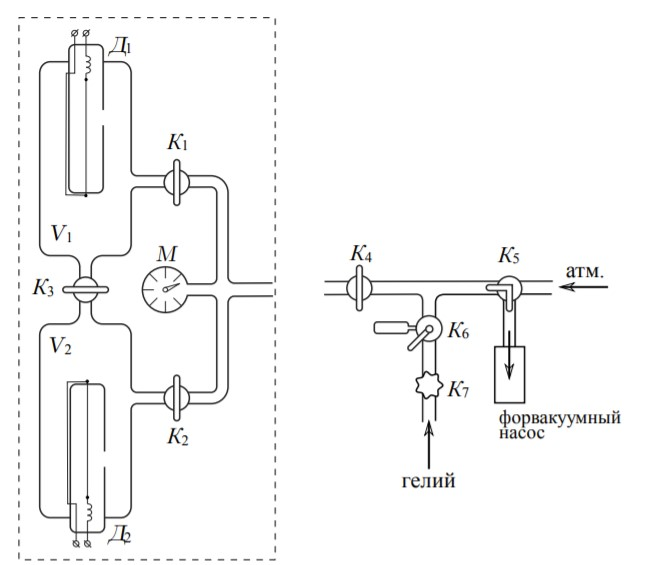
\includegraphics[width=12cm]{Схема}
	\end{center}
	\caption{Схема установки}
	\label{img2}
\end{figure}	
	

\subsection*{Ход работы}

\input{Данные}

Проведя измерения, занесем точки в таблицу \ref{tab:data}. Построим графики полученных зависимостей (см. рис. \ref{fig:pot}). 


\begin{table}
\input{Линеаризация}
\hspace{\fill}
\input{Линеаризация2}
\end{table}



\begin{figure}
	\centering
	\includegraphics[width=1\linewidth]{"P(T)"}
	\caption{Температура от давления}
	\label{fig:pot}
\end{figure}

\begin{figure}
	\centering
	\includegraphics[width=1\linewidth]{"lnP(T)"}
	\caption{Линеаризация $\ln{P}(\frac{1}{T})$}
	\label{fig:lnpot}
\end{figure}

\begin{figure}
	\centering
	\includegraphics[width=1\linewidth]{"dpdt"}
	\caption{Линеаризация $\frac{dP}{dT}(\frac{P}{T^2})$}
	\label{fig:dpdt}
\end{figure}



\begin{table}
	\caption{Обработка $\ln{p}(\frac{1}{T})$}
	\label{tab:stat}
	\centering
	\footnotesize
	\begin{tabular}{l|ccccccccc}
		\toprule
		$ $ & $\overline{x}$ & $\sigma_x^2$ & $\overline{y}$ & $\sigma_y^2$ & $r_{xy}$ & $A$ & $\Delta A$ & $B$ & $\Delta B$ \\ \midrule
		Нагрев & 3.23e-03 & 7.05e-09 & 3.74 & 2.24e-01 & -3.97e-05 & -5637.28 & 34.92 & 21.93 & 0.11 \\ 
		Охлаждение & 3.24e-03 & 8.14e-09 & 3.73 & 2.29e-01 & -4.32e-05 & -5302.52 & 29.12 & 20.90 & 0.09 \\ \bottomrule
	\end{tabular}
\end{table}


\begin{table}
	\caption{Обработка $\frac{dP}{dT}(\frac{P}{T^2})$}
	\label{tab:dpstat}
	\centering
	\footnotesize
	\begin{tabular}{l|ccccccccc}
		\toprule
		$ $ & $\overline{x}$ & $\sigma_x^2$ & $\overline{y}$ & $\sigma_y^2$ & $r_{xy}$ & $A$ & $\Delta A$ & $B$ & $\Delta B$ \\ \midrule
		Нагрев & 4.51e-04 & 2.94e-08 & 2.65 & 8.54e-01 & 1.57e-04 & 5342.85 & 211.66 & 0.24 & 0.10 \\ 
		Охлаждение & 4.95e-04 & 3.48e-08 & 2.48 & 8.01e-01 & 1.61e-04 & 4620.80 & 371.61 & 0.19 & 0.20 \\ \bottomrule
	\end{tabular}
\end{table}


Перейдем к расчету зависимостей. Обработку проведем методом наименьших квадратов:

$$y = Ax + B,$$

где $$A = \frac{r_{xy}}{ \sigma_x^2},$$
$$B = \overline{y} - A\overline{x}.$$

Для оценки погрешностей используем следующие формулы:
$$\Delta A =  t_{n-1, p} \sqrt{\frac{1}{n-2} \left( \frac{\sigma_y^2}{\sigma_x^2} - A^2 \right)},$$
$$\Delta B = \Delta A \sqrt{\sigma_x^2 + \overline{x}^2},$$

где 
$n$ - количество измерений, $ t_{n-1, p}$ - коэффициент Стьюдента

Таким образом проведем две линеаризации (см. таблицы \ref{tab:linear} и \ref{tab:linear2}) используя зависимости:

$$\frac{dP}{dT} = \frac{L}{R} \cdot \frac{P}{T^2}$$
$$\ln{P} = -\frac{L}{R} \cdot \frac{1}{T} + C$$

Всю статистическую обработку занесем в таблицы \ref{tab:stat} и \ref{tab:dpstat}. Также построим графики зависимостей, для качественного анализа поведения (см. рис. \ref{fig:lnpot} и \ref{fig:dpdt})

Так как удельная теплота отличается от коэффициента наклона множителем, то относительная погрешность будет такой же. Откуда для молярных, а затем и удельных теплот парообразования получаем значения, которые занесем в таблицу \ref{tab:itog}. Молярная масса воды $\mu = 18.02 \frac{\text{г}}{\text{моль}}$



\subsection*{Вывод}


Из отчета видно, что на точность полученных результатов (см. таблицу \ref{tab:itog}) влияет не только ошибки проведения эксперимента, но последующая обработка: выбор зависимости для линеаризации, методы определения параметров. Во втором способе погрешность получается на порядок больше, чем в первом.


\begin{table}[H]
	\caption{Вывод}
	\label{tab:itog}
	\centering
	\footnotesize
	\begin{tabular}{l|r|r}
		\toprule
		$ $ & Нагрев, $\frac{\text{Дж}}{\text{кг}}$& Охлаждение, $\frac{\text{Дж}}{\text{кг}}$ \\ \midrule
		Линеаризация $\ln{p}(\frac{1}{T})$          & $(2.601 \pm 0.014)\e{6}$ & $(2.447 \pm 0.013)\e{6}$  \\ \midrule 
		Линеаризация $\frac{dP}{dT}(\frac{P}{T^2})$ & $(2.46 \pm 0.09)\e{6}$ & $(2.13 \pm 0.17)\e{6} $  \\ \midrule
		Табличная величина 							& $2.30\e{6} $ & $2.30\e{6} $  \\ 
		\bottomrule
	\end{tabular}
\end{table}

Учесть погрешность определения теплоемкостей в данном случае проблематично, т.к. метод наименьших квадратов дает значение ошибки именно случайную. А в случае с первой линеаризацией видно, что решающую роль должна иметь систематическая погрешность измерений.


Тем не менее полученные результаты более чем подтверждают теоретическую модель. Графики получаются линейными, а значения теплоты не сильно отличаются от табличных.
 



\end{document}